\begin{figure}[h]
    \fbox{
    \begin{minipage}{\dimexpr\textwidth-2\fboxsep-2\fboxrule\relax}
        \centering
        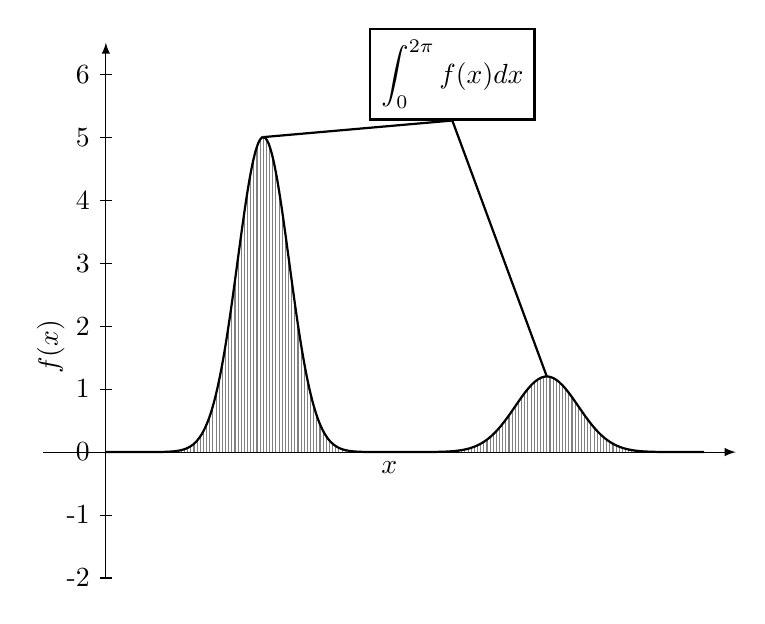
\begin{tikzpicture}[
            scale=0.8,
            declare function={ myfunc(\x) = 5*exp(-(\x-2.5)^2 * 3) + 1.2*exp(-(\x-7)^2 * 2);}
                           ]
            % 1. Draw the axes
            \draw[-latex] (-1, 0) -- (10,0.0) node[below, midway] {$x$};
            \draw[-latex] ( 0,-2) -- ( 0,6.5) node[midway, left, xshift=-7mm, rotate=90] {$f(x)$};

            % 2. Add ticks and labels to the y-axis
            \foreach \y in {-2,...,6} {
                \draw (0.1, \y) -- (-0.1, \y) node[left] {\y};
            }

            % 3. Shade the area under the first peak with vertical lines
            % This replicates the style of the original figure.
            \foreach \x in {1, 1.05, ..., 4} {
                \draw[thin, gray] (\x, 0) -- (\x, {myfunc(\x)});
            }
            % Shading for the second peak
            \foreach \x in {5.5, 5.55, ..., 8.5} {
                \draw[thin, gray] (\x, 0) -- (\x, {myfunc(\x)});
            }

            % 4. Plot the function curve
            \draw[thick, domain=0:9.5, samples=200, smooth] plot (\x, {myfunc(\x)});

            % 5. Create the box with the integral formula
            \node[draw, thick, fill=white, inner sep=4pt] (integral_box) at (5.5, 6) {$\displaystyle \int_{0}^{2\pi}f(x)dx$};

            % 6. Draw the line pointing from the box to the curve's peak
            \draw[thick] (integral_box.south) -- (2.5, 5);
            \draw[thick] (integral_box.south) -- (7, 1.2);

        \end{tikzpicture}
    \end{minipage}
    }
    \caption{\textit{The integral of a function is the area under the curve.}}
    \label{fig:08_01}
\end{figure}